\begin{table*}[ht]
\centering
\begin{minipage}{0.95\textwidth}
\centering
\small
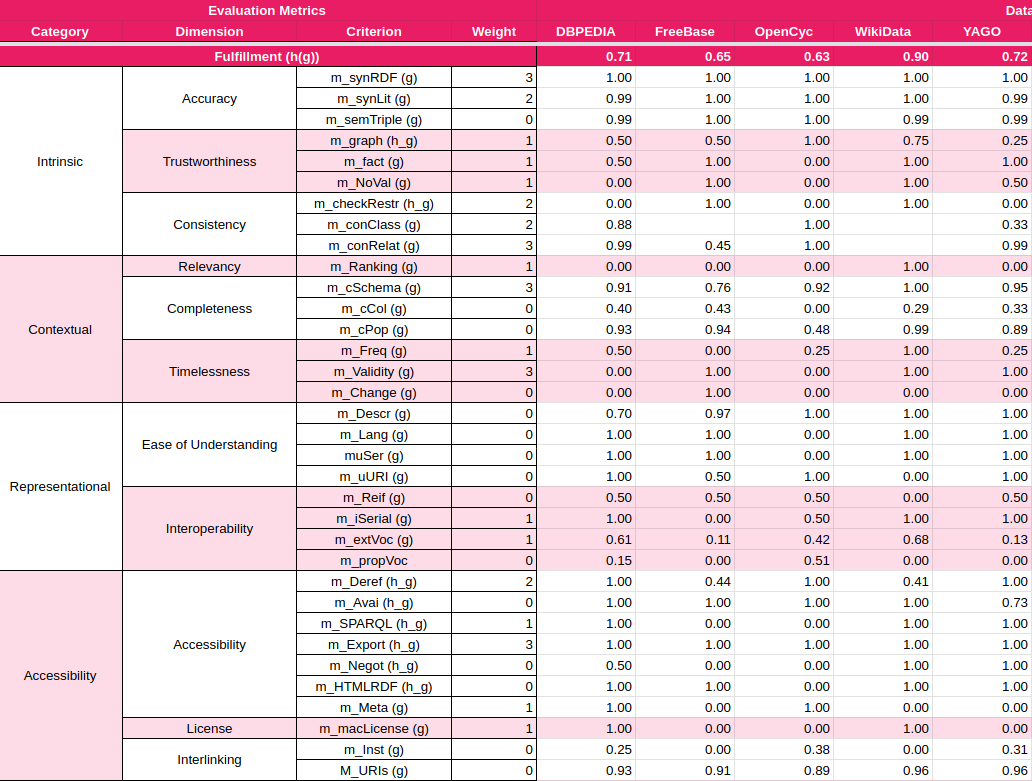
\includegraphics[scale=0.5]{content/appendix/figures/image.png}
\caption{Values for DBPEDIA, FreeBase, OpenCyc, WikiData and YAGO are taken from \cite{farber2017dataquality} as a rule. Exceptions are marked with '*' and explained in \autoref{app:kg_selection_framework}.
%Values for WordNet, ICEWS and GDELT are added \missing
}
\renewcommand{\arraystretch}{1.2}

\begin{comment}
\begin{tabular}{|m{2.5cm}|M|c|c|c|c|M|c|}
\hline
\thead{Method} & %method
\thead{Category} & %category
\thead{Temporal\\Information} & %temporal
\thead{Symmetric\\Relations} & %symmetry
\thead{Anti-\\Symmetric\\Relations} & %anti-symmetry
\thead{Entity\\Embedding} & %entity embedding
%\thead{Relation Embedding} & %relation embedding
\thead{Time\\Dimension} & %time dimension
\thead{Space} %space
\\
\hline
%\rowcolor{blue!10}
TransE \newline\cite{transe} & %method
Transformation \newline (translation) & %category
 & %temporal
 & %symmetry
\checkmark & %anti-symmetry
Separate & %entity embedding
%Single Vector & %relation embedding
\hrulefill & %time dimension
$\R$%space
\\
\hline
\end{tabular}
\end{comment}

\label{tab:selection_framework}
\end{minipage}
\end{table*}